%
%
%%%%%%%%%%%%%%%%%%%%%%%%%%%%%%%%%%%%%%%%%%%%%%%%%%%%%%%%%%%%%%%%%%%%%%%%%%%%%%%%%
% Plantilla para avance e informe final	FS0751/FS0624				%
% Traducción y adaptación del archivo:													%
% http://web.mit.edu/8.13/www/Samplepaper/sample-zipped/sample-paper.pdf 				%
%																						%
													%
% Adaptado de la página de REVTeK-4 de la American Physical Societies					%
% RECOMENDACIÓN PARA LOS ESTUDIANTES: cada vez que escriba un reporte, empiece con esta plantilla y guárdela con otro nombre. Si le es conveniente, no borre las líneas que no necesita, sino más bien coméntelas con el símbolo "%"											% En caso de tener sugerencias de mejoras puede comunicarlas al coordinador del curso, toda retroalimentación es bienvenida.								%
%%%%%%%%%%%%%%%%%%%%%%%%%%%%%%%%%%%%%%%%%%%%%%%%%%%%%%%%%%%%%%%%%%%%%%%%%%%%%%%%%


%%%%%%%%%%%%%%%%%%%%%%%%%%%%%%%%%%%%%%%%%%%%%%%%%%%%%%%%%%%%%%%%%%%%%%%%%%%%%%%%%		
% PREÁMBULO																				%
% El preámbulo en un documento LaTeX es el conjunto de comandos que preceden 			%
% la línea \begin{document} line. Contiene la línea \documentclass para cargar			%
% las definiciones REVTeK-4 y varias otras líneas \usepackage para cargar				%
% otros paquetes.																		%
%																						%
% ADVERTENCIA A LOS ESTUDIANTES: El preámbulo contiene un conjunto de paquetes necesarios para un compilado apropiado. Se recomienda no eliminar paquetes por completo aunque piense que no los necesita, coméntelos. Ud puede también agregar paquetes según lo vea conveniente.
%%%%%%%%%%%%%%%%%%%%%%%%%%%%%%%%%%%%%%%%%%%%%%%%%%%%%%%%%%%%%%%%%%%%%%%%%%%%%%%%%

\documentclass[aps,twocolumn,secnumarabic,nobalancelastpage,amsmath,amssymb,
nofootinbib]{revtex4}

% nofootinbib es otra clase de documento que permite colocar notas al pie de
% página en la página donde ocurre, en lugar de al final del artículo. De esta
% manera es más fácil de leer!

% secnumarabic es una manera particular de identificar la secciones por número.
% para ayudar a la revisión electrónica.

% amsmath and amssymb son necesarias para el ambiente de las subecuaciones, 
% entre otras

\usepackage{graphics}      % especificaciones gráficas estándar
\usepackage{graphicx}      % especificaciones alternativas para lso gráficos
\usepackage{longtable}     % ayuda con las opciones de tablas grandes
\usepackage{url}           % para referencias en línea
\usepackage{bm}            % paquete especial 'bold-math'
\usepackage[utf8]{inputenc}
\usepackage{enumitem}
\usepackage[spanish, es-tabla]{babel}% para que utilice las reglas gramaticales del español
						   % y reconozca las tildes.
						   
						   
\usepackage[letterpaper,top= 2.75cm,bottom=3.5cm,left=1.8cm,right=1.8cm]{geometry}%margenes
\usepackage{ifsym}                        %Símbolos matemáticos
\usepackage{amssymb}                      %AMS
\usepackage{amsmath}                      %AMS
\usepackage{amsthm}                       %AMS teorema
\usepackage{color}                        %LaTex Color
\usepackage{mathtools}


%\usepackage{multicol}                     %Permite escribir en columnas
%\usepackage{multirow}                                                   %Permite escribir en filas
\usepackage{multienum}                    %Permite colocar una lista en columnas
\usepackage{tabularx}                     %Permite generar tabuladores con ancho ajustables
\usepackage{booktabs}                     %Características especiales para tablas
%\usepackage{caption}    


%Cambia los caption
\usepackage{fancyhdr}
\usepackage{pgf}
\usepackage{tikz}
\tikzstyle{guiones}+=[dashed]
\usetikzlibrary{patterns,arrows,snakes,shapes,automata,plotmarks,backgrounds}
\usepackage{lscape}
\usepackage{titlesec}
\usepackage{array,ragged2e}
\newcolumntype{P}[1]{>{\RaggedRight\arraybackslash}p{#1}}
\usepackage{float}
\usepackage{lipsum}
\setlength{\columnsep}{7.5mm} 

\titleformat*{\section}{\normalsize\bfseries}
\titleformat*{\subsection}{\normalsize\bfseries}				   
						   
\def\bibsection{\section*{\refname}} 
\usepackage[pdfborder={0 0 0},colorlinks=false]{hyperref}
\usepackage{xurl} %Paquete para poder incluir enlaces largos de url en las referencias.
\usepackage{adjustbox}
%%%%%%%%%%%%%%%%%%%%%%%%%%%%%%%%%%%%%	
%                                 		%
% Y ahora, el comienzo del documento... %
%                                 		%
%%%%%%%%%%%%%%%%%%%%%%%%%%%%%%%%%%%%%
\begin{document}

% Acá se ponen los logos institucionales para la primer página del reporte.
{\begin{center}
\vskip-25pt 
{
\includegraphics[width = 175mm]{LogosInstitucionales.png}}
\end{center}}

% Título de la práctica, nombre, apellidos, carnet y correo de las personas involucradas
\title			{Implementación de una red neuronal informada por la física para la obtención de perfiles de densidad y temperatura para un plasma que presenta un transporte clásico}
\author         {Aaron Sanabria Martínez}
\email          {aaron.sanabria@ucr.ac.cr}
\author         {Ricardo Solano Piedra}
\email          {risolano@itcr.ac.cr}
\affiliation    {Escuela de Física, Universidad de Costa Rica. Sede Rodrigo Facio \\ Escuela de Física, Instituto Tecnológico de Costa Rica. Campus Cartago}
\date{\today} %la fecha sale de forma automática

%\begin{abstract}
%\lipsum[4]
%\end{abstract}

\maketitle


%%%%%%%%%%%%%%%%%%%%%%%%%%%%%%%%%%%%%%%%%%%%%%%%%%%%%%%%%%%%%%%%%%%%%%%%%%%%%%%%%
% Cada sección empieza con el comando: \section{título} 								%
%%%%%%%%%%%%%%%%%%%%%%%%%%%%%%%%%%%%%%%%%%%%%%%%%%%%%%%%%%%%%%%%%%%%%%%%%%%%%%%%%

\section{Introducción} 

El \textit{deep learning} se ha integrado en la física por su capacidad para representar funciones complejas y aprender estructuras de relaciones matemáticas \cite{carleo2019}. Dentro de estas, las redes neuronales (NNs) destacan por su capacidad para aproximar funciones, lo que las hace una opción para la resolución de sistemas diferenciales \cite{lagaris1998}.  Las redes neuronales informadas por la física (PINNs) permiten tratar sistemas complejos de ecuaciones diferenciales usando restricciones físicas para obtener soluciones. Herramientas como la autodiferenciación permiten introducir las ecuaciones diferenciales (EDs) y sus condiciones de frontera como funciones de penalización que restringen el espacio de soluciones y explotan la capacidad de aproximación de las NNs \cite{raissi2019, baydin2018}.

En el campo de plasmas se presenta no linealidad y acoplamiento en las ecuaciones que lo rigen. La dinámica de los plasmas está influenciada por interacciones electromagnéticas \cite{helander2005}. Estos sistemas son complejos debido a su comportamiento colectivo y una dinámica con múltiples regímenes de colisión que llevan al transporte de partículas \cite{goldston1995}. La descripción de fluidos del plasma da un sistema cerrado de ecuaciones diferenciales parciales (PDEs) que puede ser modelado con  una teoría de transporte clásico \cite{freidberg2014}. Pese a que estos sistemas pueden ser reducidos a uno de ecuaciones diferenciales ordinarias (ODEs) con modelos 1D, siguen siendo complejos de tratar\cite{lechte2002, alves2018}.

Los coeficientes y los términos fuentes en los sistemas de EDs que aparecen en los modelos de transporte colisional no son constantes, además de no lineales, por lo que el uso de PINNs es un buen método por su capacidad de integrar y representar la no linealidad \cite{zhong2022}. Por ejemplo, se han implementado PINNs para la resolución de ecuaciones unidimensionales del transporte de plasma a bajas temperaturas \cite{zhong2022, trieschmann2023}. Esquemas de PINNs aplicados en el transporte en Tokamaks han sido comparados con métodos tradicionales de diferencias finitas en la resolución de PDEs con beneficios como reducción en el tiempo de convergencia \cite{seo2024}. En el transporte turbulento para encontrar campos consistentes con las ecuaciones del fluido doble de Braginskii \cite{mathews2021}. Sin embargo, no se ha reportado la implementación de una PINN aplicada al transporte perpendicular en geometría cilíndrica bajo el modelo de Braginskii reducido a ODEs con coeficientes dependientes de los perfiles.

No se ha reportado el uso de PINNs para el caso del transporte perpendicular para una geometría cilíndrica en la solución de las ecuaciones de fluido de Braginskii como un problema de ODEs con coeficientes dependientes de los perfiles. Las PINNs integran la no linealidad y la física al problema directamente en las funciones de pérdida usando la autodiferenciación (AD) sin uso de grillas. 
\section{Pregunta de investigación}
La pregunta que se plantea contestar es: ¿puede una PINN, basada únicamente en restricciones físicas, reproducir perfiles radiales de densidad y temperatura en un plasma magnetizado bajo transporte clásico con un nivel de precisión comparable a datos experimentales del dispositivo de fusión Rijnhuizen Tokamak Project (RTP)?
\section{Objetivo general}
Implementar una Red Neuronal Informada por la Física (PINN) para la determinación de los perfiles radiales de densidad electrónica y temperatura electrónica en un plasma magnetizado cilíndrico que exhibe transporte clásico perpendicular al campo magnético.
\vspace{- 4 mm}
\subsection*{Objetivos específicos}
\vspace{- 4 mm}
\begin{enumerate}[noitemsep]
			\item Formular las ecuaciones que relacionan la densidad electrónica y temperatura electrónica a partir de la teoría de transporte clásico perpendicular al campo magnético para la base del diseño de la PINN.
			\item Diseñar la arquitectura de la PINN de acuerdo al modelo teórico mediante la definición de las capas, las funciones de activación y los hiperparámetros esenciales de la red. 
			\item  Evaluar cuantitativamente la precisión de la PINN mediante la comparación con perfiles experimentales del RTP utilizando métricas como error cuadrático medio (MSE) y análisis de consistencia física.
		\end{enumerate}
%%%%%%%%%%%%%%%%%%%%%%%%%%%%%%%%%%%%%%%%%%%%%%%%%%%%%%%%%%%%%%%%%%%%%%%%%%%%%%%%%%%%%%%%%%%%%%%%%%%%%%%%%%%%%%
\vspace{-4 mm}
\section{Marco teórico}

\subsection{Redes neuronales informadas por la física: fundamentos}

Las \textbf{neuronas} artificiales son funciones matemáticas y son la estructura básica de las NNs. Las neuronas se conectan entre sí usando capas que toman como argumentos vectores de salida de las capas previas. Los perceptrones multicapa (MLP) son una NN completamente conectada donde la información fluye únicamente de la capa de entrada a la capa de salida,  sin ciclos ni retroalimentación, i.e., $\mathcal{F} : X \rightarrow Y \quad \text{con} \quad \mathcal F = f^{(L)} \circ f^{(L-1)} \circ \dots \circ f^{(1)}$ con $X$ es el espacio de entradas y $Y$ el espacio de salidas. Cada capa aplica una transformación afín seguida de una activación no lineal por la función $\sigma(\cdot)$ que debe ser diferenciable.
\begin{equation}
	f^{(k)}(\bm{x}_{k-1})  = \sigma(\bm{W}^{(k)}\bm{x}_{k -1 } + \bm{b}^{(k)})
\end{equation}
 donde $\bm{W}^{(k)}$ es una matriz de pesos y  $\bm{b}^{(k)}$ el sesgo, son parámetros de la NN que se ajustan durante el entrenamiento. Una función general continua puede ser aproximada con precisión arbitraria usando MLPs \cite{cybenko1989, hornik1989}.
 
En la Figura \ref{fig:mpl} se muestra el esquema general de lo que es un MLP.
\begin{figure}[htb]
	\centering
	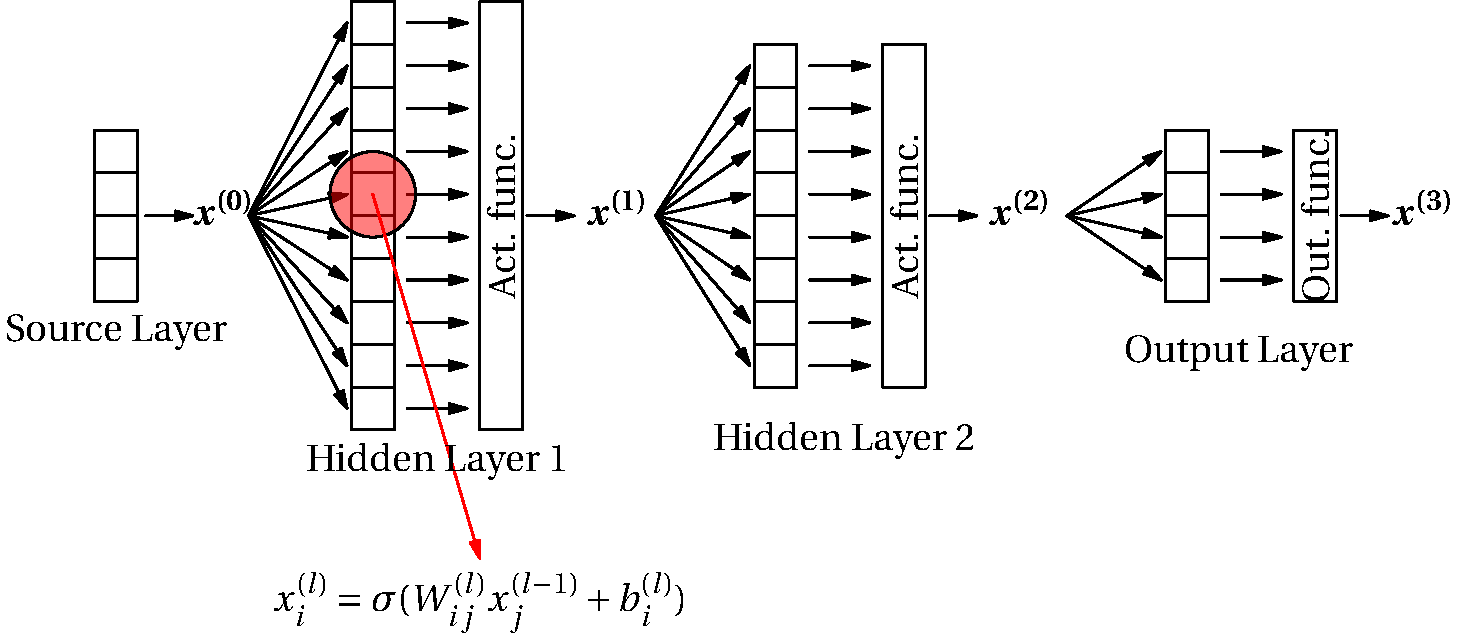
\includegraphics[width = 0.5\textwidth]{figures/MLP.pdf}
	\caption{MLP con dos capas ocultas. Adaptado de \cite{ray2023} bajo licencia CC BY-NC-SA 4.0.}
	\label{fig:mpl}
\end{figure}

Las entradas, salidas y transformaciones en las NNs se guardan en tensores que almacenan los parámetros e hiperparámetros de la MLP, así como el grafo de cómputo de las operaciones sobre ellos y sus derivadas locales. Esto da paso al método AD que parte del principio de que toda operación computacional puede ser descompuesta en operaciones elementales con derivadas conocidas. La función de activación debe ser diferenciable en los puntos donde se aplica AD para evitar problemas con las derivadas.

\subsubsection{Funciones de pérdida}

Las funciones de pérdida $\mathcal{L}( \{x_i\}, \theta)$ cuantifican cuánto se apegan los modelos a las restricciones que se les imponen en determinados puntos $\{x_i\} \in X$  conocidos como  puntos de colocación. Durante el entrenamiento se minimiza $\mathcal{L}(\bm{\theta})$ al variar los parámetros internos del modelo $\bm{\theta} \coloneqq \{ \bm{ W}^{(k)}, \bm{b}^{(k)}\}$.  Las funciones $\mathcal{L}(\bm{\theta})$ pueden contener múltiples términos correspondientes a diferentes condiciones sobre el modelo; si se imponen sobre las EDs que rigen un sistema físico y sus condiciones de frontera, surge el concepto de PINN \cite{raissi2019}.

Las NNs requieren tanto de los parámetros $\bm{\theta}$ como de los hiperparámetros de la red $\bm{\Theta}$ que contienen el número de capas $L + 1$, el ancho de la red, la función de activación que se usa $\sigma$, etc. Una arquitectura de NN robusta requiere de una fase de entrenamiento donde se optimizan los valores de $\bm{\theta}$ dado un conjunto de $\bm{\Theta}$ fijos \cite{ray2023}.

\subsubsection{Optimizadores}

Los algoritmos de optimización modernos parten del algoritmo de descenso por gradiente (GD), donde se usa la dirección opuesta al gradiente de $\mathcal{L}(\bm{\theta})$ y un hiperparámetro llamado tasa de aprendizaje $\eta$ que es el tamaño del paso usado. Es la base de algoritmos más eficientes. 

Los algoritmos basados en GD pueden desvanecerse o explotar. Esto se previene controlando la varianza de las señales que se pasan a la NN al inicializar los parámetros con valores aleatorios de una distribución uniforme o normal. El inicializador Xavier trata las derivadas de la función de pérdida como variables aleatorias \cite{glorot2010}.

El estimador adaptativo de momentos (Adam) está basado en gradientes estocásticos de primer orden donde las $\eta$ son adaptativas. Se introducen momentos que guardan el historial del gradiente $\nabla_{\bm{\theta}} \mathcal{L}$. El método es robusto para tratar problemas dispersos y con ruido \cite{kingma2017}.

El algoritmo de memoria limitada Broyden-Fletcher-Goldfarb-Shanno (L-BFGS) es un método de memoria cuasi-newtoniano de segundo orden que estima la matriz hessiana de $\mathcal{L}(\bm{\theta})$ respecto a los parámetros sin calcular todos los elementos de la matriz, cerca de un mínimo la convergencia es más rápida que en métodos de primer orden. 
%%%%%%%%%%%%%%%%%%%%%%%%%%%%%%%%%%%%%%%%%%%%%%%%%%%%%%%%%%%%%%%%%%%%%%%%%%%%%%%%%%%%%%%%%%%%%%%%%%%%%%%%%%%%%%%%%%%%%%%%%%%%%%%%%%%%%%%%

\subsection{Plasmas magnetizados y teoría clásica de transporte perpendicular}

Un plasma es un gas ionizado que presenta comportamiento colectivo y cuasi-neutralidad. La dinámica del plasma está gobernada por interacciones electromagnéticas de largo alcance tanto por campos que se generan a nivel interno como por campos exteriores. La teoría de transporte colisional estudia el transporte de partículas, momento y energía  en un régimen dominado por colisiones. Cuando partículas, momento y energía se transportan en dirección perpendicular a un campo magnético establecido en el plasma, se alude al concepto de transporte perpendicular. La teoría de transporte clásico estudia la contribución de las colisiones al transporte perpendicular en un plasma magnetizado \cite{helander2005}.

\subsubsection{Ecuación cinética de Boltzmann}

Una descripción estadística asume que hay suficientes partículas en el sistema para tener una descripción macroscópica con temperatura y densidad bien definidas. Se trabaja en un espacio de fase 6-dimensional $(\bm{x}, \bm{v})$. Primero se introduce el operador $d/dt $ como
\begin{equation}
	\frac{d}{dt} \equiv \partial_t + \textbf{v}\cdot\nabla + \frac{Z_\alpha e}{m_\alpha}(\textbf{E} + \textbf{v}\times\textbf{B})\cdot \nabla_\textbf{v}
\end{equation}
este operador toma en cuenta la evolución temporal local, la advección espacial y la interacción electromagnética con campos externos. Las especies en un plasma pueden ser especificadas por una función de distribución $f_\alpha(\bm{x}, \bm{v}, t)$ mediante la siguiente ecuación:
 \begin{equation}\label{eq:boltzmanngleichung}                                                                                          
    \left[\frac{d}{dt} - C_{\alpha,\beta}\right]f_\alpha = 0
  \end{equation}
en este caso $C_{\alpha, \beta}$ es un operador de colisiones binarias entre especies $\alpha$ y $\beta$ que describe colisiones que se dan en el medio.

Al integrar la ecuación \eqref{eq:boltzmanngleichung} respecto al espacio de velocidades con pesos $g_k$ correctos, se puede obtener la descripción de fluidos en el plasma al tomar los momentos $k=0$ y $k=2$. La ecuación \eqref{eq:partflux} describe el flujo de partículas de plasma a partir de $g_0$
\begin{equation}\label{eq:partflux}
	\partial_t n_\alpha + \nabla\cdot\bm{\Gamma}_\alpha = S_\alpha
\end{equation}
con $n_\alpha$ y $\bm{u}_\alpha$ la densidad y velocidad promedio del plasma respectivamente, $\bm{\Gamma}_\alpha = n_\alpha\bm{u}_\alpha$ el flujo de partículas y $S_\alpha$ un término de fuentes y sumideros. Por otro lado, la ecuación \eqref{eq:energy}, que describe el flujo de energía en el plasma, se obtiene a partir de $g_2$ 
\begin{eqnarray}\label{eq:energy}
	\partial_t W_\alpha + \nabla\cdot\bm{Q}_\alpha =  P_\alpha
\end{eqnarray}
con $W_\alpha$ la densidad de energía del sistema, $\bm{Q}_\alpha$ el flujo de energía y $P_\alpha$ términos de potencia y disipación de energía \cite{helander2005, freidberg2014}. 

\subsubsection{Colisiones y procesos atómicos en el plasma}

Los términos de fuente y sumideros en las ecuaciones \eqref{eq:partflux} y \eqref{eq:energy} se relacionan con procesos atómicos y pueden modelarse como \cite{goldston1995}
\begin{eqnarray}
	S_\text{proceso} &=& n_\alpha n_\beta \langle \sigma v \rangle_\text{proceso}\\
	P_\text{proceso} &=& E_\text{proceso} n_\alpha n_\beta \langle \sigma v \rangle_\text{proceso} 
\end{eqnarray}

donde $\sigma$ es la sección efectiva de la colisión. Los términos de fuente y sumidero de partículas así como la energía dependen de $\langle \sigma v\rangle$, la tasa a la cual ocurren las colisiones que dan lugar al proceso atómico.  

\subsubsection{Procesos de calentamiento en el plasma}

En los procesos de calentamiento se debe considerar el esfuerzo viscoso en el plasma $\bm{\Pi}_\alpha$ y la presión mecánica $p_\alpha$. El flujo de calor $\bm{Q}_\alpha$ puede dividirse en diferentes contribuciones tal que

\begin{equation}\label{eq:heatflux}
    \textbf{Q}_\alpha = \textbf{q}_\alpha + \frac{3}{2}T_\alpha\pmb{\Gamma}_\alpha + p_\alpha\textbf{u}_\alpha + \pmb{\Pi}_\alpha\cdot\textbf{u}_\alpha + \frac{1}{2}m_\alpha u_\alpha^2\pmb{\Gamma}_\alpha
  \end{equation}
 
 Las diferentes contribuciones de flujos corresponden en orden a: calentamiento conductivo, convectivo, la entalpía o trabajo que hace la presión mecánica sobre el plasma, el transporte viscoso de energía y la convección de energía cinética \cite{helander2005}. Bajo ciertos supuestos es posible despreciar algunas de estas contribuciones. 
 
 \subsubsection{Parámetros característicos del plasma}
 
 El radio de Debye $\lambda_D = \sqrt{\epsilon_0 T / n_e e^2}$ es una distancia en la que el potencial de Coulomb se ve apantallado por el comportamiento colectivo de las partículas. Con $\lambda_D$ y el parámetro de impacto mínimo $b_\text{min}$ se define la cantidad $\Lambda \equiv \lambda_D/ b_\text{min} = 4\pi \epsilon^{3/2} e^{-3} T_e^{3/2} n_e^{-1/2}$ \cite{goldston1995, helander2005}. Se define el tiempo de relajación $\tau_{\alpha, \beta}$ que es el periodo típico entre colisiones electrónicas
\begin{equation*}
	\tau_{e, i}^{-1} = \left(\frac{e^2}{4\pi\epsilon_0}\right)^2 \frac{8\sqrt{2\pi m_e n_e}}{3 m_i}\frac{\ln{\Lambda}}{T_e^{3/2}}
\end{equation*}
En el plasma se da difusión de partículas y energía. Para un plasma cilíndrico con $\bm{B}$ uniforme y presión constante, los flujos tienen la forma \cite{helander2005}
\begin{eqnarray}\label{eq:diffusion}
	\bm{\Gamma}_e \approx -D_\perp(n_e, T_e) \partial_r n_e \quad \text{con} \quad D_\perp = \frac{T_e}{m_e \omega_e^2 \tau_{ei} } \\
	\bm{q}_e \approx -\chi_\perp(n_e,T_e) \partial_r T_e \quad \text{con} \quad \chi_\perp = 4.66\frac{n_eT_e}{m_e \omega_e^2 \tau_{ei} } 
\end{eqnarray}
con $\omega_e$ es la frecuencia ciclotrónica del electrón. 
%%%%%%%%%%%%%%%%%%%%%%%%%%%%%%%%%%%%%%%%%%%%%%%%%%%%%%%%%%%%%%%%%%%%%%%%%%%%%%%%%%%%%%%%%%%%%%%%%%%%%%%%%%%%%%%%%%%%%%%%%%%%%%%%%%%%%%%%
%%%%%%%%%%%%%%%%%%%%%%%%%%%%%%%%%%%%%%%%%%%%%%%%%%%%%%%%%%%%%%%%%%%%%%%%%%%%%%%%%%%%%%%%%%%%%%%%%%%%%%%%%%%%%%%%%%%%%%%%%%%%%%%%%%%%%%%%
\section{Metodología}

Para la derivación teórica de las ecuaciones que determinan los perfiles de densidad $n$ y temperatura $T$ electrónicos, se parte de las ecuaciones \eqref{eq:partflux}, \eqref{eq:energy} y de los siguientes supuestos:
\begin{itemize}[noitemsep]
\item Cuasi-neutralidad: $n_i \approx n_e$.
\item Plasma débilmente ionizado: $n_e \ll n_0$.
\item Plasma frío: $T_i \ll T_e$.
\item Caso estacionario con difusión ambipolar $\bm{\Gamma}_i \approx \bm{\Gamma}_e$.
\item Geometría cilíndrica del plasma con transporte en la dirección radial: $T_e = T_e(r)$, $n_e = n_e(r)$.
\item La temperatura y densidad son continuas y diferenciables a lo largo del plasma.
\item Campo magnético $\bm{B}$ uniforme en la dirección $\hat{z}$ y campo eléctrico externo $\bm{E} = \bm{0}$.
\item La densidad de neutros es aproximadamente uniforme en el espacio $n_0 \approx \text{constant}$.
\item La deposición de potencia en el plasma sigue un perfil gaussiano $P(r) = P_\text{ext} \mathcal{N}(r; \mu, \sigma) / N$ normalizado por $N$ . 
\item El flujo de energía está dominado por convección y conducción: $\bm{Q} \approx \bm{q} + \frac{3}{2}T\bm{\Gamma}$
\end{itemize}
A partir de ahora se omitirá la etiqueta $\alpha$ que caracteriza la especie. Se llegará a un sistema de ODEs donde los perfiles serán normalizados respecto a $n_\text{max}$ y $T_\text{max}$ asumiendo que los perfiles alcanzan su máximo en el centro del plasma. El sistema resultante es de la forma
\begin{equation}\label{eq:odesys}
	\begin{cases}
		F(r, \partial_r \hat{n}, \partial_r \hat{T}, \partial_r^2 \hat{n}, \partial_r^2\hat{T}, \bm{\Psi}) = 0, \quad r \in [0, R]\\
		G(r, \partial_r \hat{n}, \partial_r \hat{T}, \partial_r^2 \hat{n}, \partial_r^2\hat{T}, \bm{\Psi}) = 0, \\
		\hat{n}(0) - 1 = 0, \quad \partial_r \hat{n}\big{|}_{r = 0} = 0, \\
		\hat{T}(0) - 1 = 0, \quad \partial_r \hat{T}\big{|}_{r = 0} = 0,\\
		\partial_r \hat{n} \big{|}_{r = R} + \hat{n}(R)/\lambda_n = 0\\
		\partial_r \hat{T} \big{|}_{r = R}  + \hat{T}(R)/\lambda_T = 0
	\end{cases}
\end{equation}

donde $\lambda_n$ y $\lambda_T$ son las escalas características de decaimiento en $r = R$ y con $\bm{\Psi} = \{R, B, n_0, P_\text{ext}, \lambda_n, \lambda_T, \mu, \sigma\}$ el conjunto de parámetros libres del sistema. $R$, el radio del plasma cilíndrico. Las condiciones en $r = 0$ corresponden a la simetría axial del sistema. El orden dos es de esperar por las ecuaciones \eqref{eq:diffusion}
\subsection{Implementación de la red}
Se construirá una MLP inicializada con Xavier activada por una función $\tanh$. Consistirá en una capa de entrada $r$, múltiples capas ocultas $L$ y una capa de salida con dos neuronas $[\hat{n}(r; \bm{\theta}), \hat{T}(r; \bm{\theta})]$ en Python usando PyTorch \cite{pytorch} para construir la PINN. Se entrenará con GPUs del clúster de la Universidad de Costa Rica. Las funciones de pérdida serán puramente físicas de la forma \cite{raissi2019}:
\begin{equation}
	\mathcal{L}(r; \bm{\theta}) = \omega_\mathcal{N} \mathcal{L}_\mathcal{N} (r; \bm{\theta})+ \omega_{bc} \mathcal{L}_{bc}(r; \bm{\theta})
\end{equation}
con
{\small
\begin{eqnarray}
	\mathcal{L}_\mathcal{N} (r; \bm{\theta}) &=&\frac{1}{N_\mathcal{N}}\sum\limits_{I=1}^{N_\mathcal{N}} || \mathcal{N}(r, \partial_r \hat{n}, \partial_r \hat{T}, \partial_r^2 \hat{n}, \partial_r^2\hat{T}, \bm{\Psi}) ||_2^2\\
	\mathcal{L}_{bc}(r; \bm{\theta}) &=& \frac{1}{N_{bc}}\sum\limits_{i=1}^{N_{bc}} || f_{bc}(r_0)||_2^2
\end{eqnarray}}
aquí $N_i$ y $\omega_i$ son los puntos de colocación y pesos  para las funciones de pérdida respectivamente que determinarán experimentalmente junto con $L$ para mejorar la convergencia . $\mathcal{L}_\mathcal{N}$ corresponde a la contribución de la restricción impuesta por las ODEs  $\mathcal{N} = (F,G)$ y sus condiciones de frontera $\mathcal{L}_{bc}$ por $f_{bc}(r_0) = 0$ evaluadas en los extremos $r_0 = 0$ y $r_0 = R$.

Para optimizar los parámetros PINN se usará el esquema de dos optimizadores. Una primera optimización con Adam seguida de un refinamiento usando L-BFGS.

Dentro de \eqref{eq:odesys} aparecen términos de disipación de energía y partículas relacionadas con las tasas $\langle \sigma v \rangle$, estas dependen de la temperatura y se determinan numéricamente de la base de datos ADAS con la librería \textit{Cherab v1.5} \cite{cherab} para un gas de hidrógeno usado en los disparos elegidos del tokamak RTP.
\vspace{- 5 mm}
\subsubsection{Críterio de convergencia}
\vspace{- 2 mm}
Se utilizará como métrica principal el error cuadrático medio (MSE)
\vspace{- 3 mm} 
\begin{equation}
MSE = \frac{1}{n}\sum\limits_{i = 1}^m(y_i - \hat{y}_i)^2
\end{equation}
donde se compararán los perfiles medidos para RTP con los obtenidos de la PINN. A partir de una tolerancia en la pérdida, estabilidad del entrenamiento, comparación del perfil radial, error relativo y comportamiento físico (monotonía, regularidad) con los que se calibrarán los hiperparámetros de la red. Aún se está valorando si la calibración será manual o se usará algún método como la interferencia bayesiana.
\vspace{- 5 mm}
\subsection{Obtención de datos para comparar perfiles}
A partir de $n(r)$ y $T(r)$ de la PINN se compararán con perfiles medidos para el dispositivo RTP en los disparos $\#96040237$, $\#97052261$ y $\#97053056$. Se promediarán temporalmente para obtener perfiles estacionarios. Los datos serán obtenidos de la base de datos IMDB \cite{roach2008} usando MDSPlus \cite{stillerman1997}.
\vspace{- 6 mm}
\section{Cronograma}
\vspace{-10mm}
\begin{table}[h!]
\caption{Cronograma de trabajo para el proyecto de investigación.}
\label{tab:cronograma}
\resizebox{0.45\textwidth}{!}{
\begin{tabular}{|l|l|}
\hline
\textbf{Semana}          & \textbf{Actividad}                                                                                                \\ \hline
09 - 27 de marzo & \begin{tabular}[c]{@{}l@{}}Revisión bibliográfica / Escritura de Anteproyecto / \\ Derivación de las ecuaciones del modelo\end{tabular}      \\ \hline
06 - 10 de abril         & Entrenamiento en la implementación de PINNs                                                                       \\ \hline
13 de abril - 01 de mayo & \begin{tabular}[c]{@{}l@{}}Redacción del Avance /\\ construir la arquitectura de la PINN\end{tabular}             \\ \hline
04 - 15 de mayo          & \begin{tabular}[c]{@{}l@{}}Redacción del Avance / \\ Probar y Ajustar la PINN/\end{tabular}                       \\ \hline
15 - 22 de mayo  & \begin{tabular}[c]{@{}l@{}}Terminar Avance / obtener y definir los perfiles a usar  \\ de la base de datos/ Trabajar en la PINN\end{tabular} \\ \hline
22 de mayo - 12 de junio & \begin{tabular}[c]{@{}l@{}}Comparar resultados de la PINN con \\ perfiles de la base de datos.\end{tabular}       \\ \hline
15 - 03 de junio         & \begin{tabular}[c]{@{}l@{}}Redacción del Informe Final / \\ Análisis de resultados\end{tabular}                   \\ \hline
06 - 10 de Julio         & \begin{tabular}[c]{@{}l@{}}Trabajar en la presentación y póster/ \\ Correcciones en el informe final\end{tabular} \\ \hline
\end{tabular}}
\end{table}
\vspace{- 6 mm}
\section{Uso de inteligencia artificial}
\vspace{- 3 mm}
Se usó la LLM Claude para búsqueda bibliográfica, revisión ortográfica y estructural del texto. Se usará para \textit{debugging} de código.

%%%%%%%%%%%%%%%%%%%%%%%%%%%%%%%%%%%%%%%%%%%%%%%%%%%%%%%%%%%%%%%%%%%%%%%%%%%%%%%%%
% Se puede citar un libro o un artículo con el comando: \cite{referencia}.				%
% Las referencias serán definidas en la bibliografía al final de este archivo .tex, en este plantilla está como sample-paper.bib																		%
% Se puede hacer referencia a tablas, figuras y ecuaciones usando el 					%
% comando: \ref{etiqueta}. Cada tabla y cada figura necesita una etiqueta única.		%
%%%%%%%%%%%%%%%%%%%%%%%%%%%%%%%%%%%%%%%%%%%%%%%%%%%%%%%%



%%%%%%%%%%%%%%%%%%%%%%%%%%%%%%%%%%%%%%%%%%%%%%%%%%%%%%%%%%%%%%%%%%%%%%%%%%%%%%%%%
%%%%%%%%%%%%%%%%%%%%%%%%%%%%%%%%%%%%%%%%%%%%%%%%%%%%%%%%%%%%%%%%%%%%%%%%%%%%%%%%%


% ... si se necesita se puede insertar un salto de línea con dos backslashes: \\


%%%%%%%%%%%%%%%%%%%%%%%%%%%%%%%%%%%%%%%%%%%%%%%%%%%%%%%%%%%%%%%%%%%%%%%%%%%%%%%%%
% Asegúrese de que no haya línea vacía despues de \end{equation} y antes de las			%
% siguientes líneas, si no lo hace así, se comenzará como un nuevo párrafo.				%
%%%%%%%%%%%%%%%%%%%%%%%%%%%%%%%%%%%%%%%%%%%%%%%%%%%%%%%%%%%%%%%%%%%%%%%%%%%%%%%%%


%%%%%%%%%%%%%%%%%%%%%%%%%%%%%%%%%%%%%%%%%%%%%%%%%%%%%%%%%%%%%%%%%%%%%%%%%%%%%%%%%


%%%%%%%%%%%%%%%%%%%%%%%%%%%%%%%%%%%%%%%%%%%%%%%%%%%%%%%%%%%%%%%%%%%%%%%%%%%%%%%%%
%%%%%%%%%%%%%%%%%%%%%%%%%%%%%%%%%%%%%%%%%%%%%%%%%%%%%%%%%%%%%%%%%%%%%%%%%%%%%%%%%


%%%%%%%%%%%%%%%%%%%%%%%%%%%%%%%%%%%%%%%%%%%%%%%%%%%%%%%%%%%%%%%%%%%%%%%%%%%%%%%%%
% Así es como se define una tabla: [!hbt] significa que LaTeX está forzado				%
% (por medio del !) a colocar la tablar aquí (h:here), o si eso no fuciona porque		%
% no existe el espacio necesario, LaTeX intentará colocarla al final de la página		%
% (b:bottom) o al principio (t:top).	
%%%%%%%%%%%%%%%%%%%%%%%%%%%%%%%%%%%%%%%%%%%%%%%%%%%%%%%%%%%%%%%%%%%%%%%%%%%%%%%%%


%%%%%%%%%%%%%%%%%%%%%%%%%%%%%%%%%%%%%%%%%%%%%%%%%%%%%%%%%%%%%%%%%%%%%%%%%%%%%%%%%
%%%%%%%%%%%%%%%%%%%%%%%%%%%%%%%%%%%%%%%%%%%%%%%%%%%%%%%%%%%%%%%%%%%%%%%%%%%%%%%%%


%%%%%%%%%%%%%%%%%%%%%%%%%%%%%%%%%%%%%%%%%%%%%%%%%%%%%%%%%%%%%%%%%%%%%%%%%%%%%%%%%
% Coloque todas las referencias usadas en este artículo en un archivo					%
% con el mismo nombre que lleva el comando \bibliography 								%
%%%%%%%%%%%%%%%%%%%%%%%%%%%%%%%%%%%%%%%%%%%%%%%%%%%%%%%%%%%%%%%%%%%%%%%%%%%%%%%%%
%%%%%%%%%%%%%%%%%%%%%%%%%%%%%%%%%%%%%%%%%%%%%%%%%%%%%%%%%%%%%%%%%%%%%%%%%%%%%%%%%
% Ahora añadimos el archivo fuente de la bobliografía(sin incluir el .bib)				% 
%%%%%%%%%%%%%%%%%%%%%%%%%%%%%%%%%%%%%%%%%%%%%%%%%%%%%%%%%%%%%%%%%%%%%%%%%%%%%%%%%
%\bibliography{sample-paper}
\bibliography{references}
\bibliographystyle{apsrev4-1}

%%%%%%%%%%%%%%%%%%%%%%%%%%%%%%%%%%%%%%%%%%%%%%%%%%%%%%%%%%%%%%%%%%%%%%%%%%%%%%%%%
%%%%%%%%%%%%%%%%%%%%%%%%%%%%%%%%%%%%%%%%%%%%%%%%%%%%%%%%%%%%%%%%%%%%%%%%%%%%%%%%%
% Otra manera de poner la bibliografía:													%
%																						%
%\bibliographystyle{prsty}																%
%\begin{thebibliography}{99}															%
%\bibitem{melissinos1966}Melissinos, A.C., Experiments in Modern						%
%  Physics - 1st Edition, Academic Press,  [1966]										%
%\bibitem{melissinos2003}Melissinos, A.C., Napolitano, J.,  Experiments in Modern		%
%  Physics - 2nd Edition, Academic Press,  [2003]										%
%\bibitem{bevington2003}Bevington and Robinson, Data Reduction and						%
%  Error Analysis for the Physical Sciences - 3rd Edition, McGraw-Hill,					%
%  [2003]																				%
%\bibitem{pritchard1990}Professor D. Pritchard, Personal Communication					%
%\end{thebibliography}																	%
																						%
%%%%%%%%%%%%%%%%%%%%%%%%%%%%%%%%%%%%%%%%%%%%%%%%%%%%%%%%%%%%%%%%%%%%%%%%%%%%%%%%%
%%%%%%%%%%%%%%%%%%%%%%%%%%%%%%%%%%%%%%%%%%%%%%%%%%%%%%%%%%%%%%%%%%%%%%%%%%%%%%%%%

\clearpage
\appendix


\end{document}
